\documentclass[12pt,a4paper]{article}
% This text is inserted in the beginning of all
% LaTex and Tex files I create.
%
% File created: Tue Sep 26 2017
% File name:    report_template.tex
% Path:         /home/name/Classes/AMPIII/Template/
%
% Name
% Sept, 2017
%
% !TEX root = ./main/file.tex
%recommended by fancyhdr package
\setlength{\headheight}{14.49998pt}
\addtolength{\topmargin}{-2.49998pt}

% include a minimal set of useful packages
\usepackage{graphicx}
\usepackage{amsfonts} 
\usepackage{amssymb}
\usepackage{amsmath}
\usepackage[a4paper,margin=4cm]{geometry}
\usepackage{lastpage}
\usepackage{fancyhdr}
\usepackage{float}
 
% PUT YOUR TITLE AND NAME HERE
\newcommand{\titlestr}{Modelling the Outcome of Tennis Matches \\ Interim Report}
\newcommand{\shorttitlestr}{Modelling Tennis Outcomes}
\newcommand{\authorstr}{S. Gilbert} % INSERT YOUR NAME(S)

\begin{document}
%%%%%%%%%%%%%%%%%%%%%%%%%%%%%%555
% title page
\begin{titlepage}
  \centering

  {\LARGE \titlestr \par}

  \vspace{1cm}
  {\Large \authorstr \par}

  {\bf A1737770.}

  \vspace{1cm}
  \today     % PUT YOUR DATE HERE

  \vspace{2cm}
  Report submitted for
    {\bf Data Science Research Project}
  at the School of Mathematical Sciences,
  University of Adelaide

  
\includegraphics[width=0.35\textwidth]{UoA_logo_col_vert.jpg}

  \vspace{2cm}
  \flushleft
  Project Area: {\bf Data Science - Modelling} \\
  Project Supervisor: {\bf Dylan Morris} \\

  \vspace{5mm} {\footnotesize In submitting this work I am indicating
    that I have read the University's Academic Integrity Policy. I
    declare that all material in this assessment is my own work except
    where there is clear acknowledgement and reference to the work of
    others.\par}

  \vspace{5mm} {\footnotesize I give permission for this work
    to be reproduced and submitted to other academic staff for
    educational purposes.\par}

  \vspace{5mm} {\footnotesize I give permission this work
    to be reproduced and provided to future students as an exemplar report.\par}

  \vfill
\end{titlepage}

% put headings on each page
\pagestyle{fancy}
\fancyhf{}
\rhead{\shorttitlestr}
\lhead{\authorstr}
\rfoot{Page \thepage\ of \pageref{LastPage}}
\renewcommand{\headrulewidth}{1pt}

%%%%%%%%%%%%%%%%%%%%%%%%%%%%%%555
% abstract
\begin{abstract}
  Tennis is a multi-billion dollar industry with the outcome of tournaments
  and individual matches having both enormous monetary ramifications' and impacts
  for player legacy.
  Accurately predicting the outcome of tennis matches under pin
  the tennis bookmaking industry. This leads to profit incentives both on
  the side of the bookmakers and on betters looking to "beat the odds".
  This report investigates various mathematical modelling methods to evaluate
  what is the best performing model when built leveraging past performance
  to determine future outcomes.

  By leveraging open-source datasets of historical tennis data, mathematical models
  can be built to predict the outcome of tennis matches. This performance was
  measured using accuracy, which is the proportion of guesses that were correct, log loss, which aims to
  measure how confident the model is in its prediction and calibration which measures
  the rate a model is likely to predict the higher ranked player to win. Alongside the data used to
  build and train these models, open source historical gambling odds were used to
  benchmark the various models performances.

  The models investigated ranged from a simple logistics model through to
  several Elo based models. The simpler logistic model use more traditional statistical
  analysis methods for deriving model parameters whereas the Elo models rely on
  predefined hyperparameters to influence the performance of the model. Comparing and
  contrasting these different approaches and their impact on prediction accuracy and
  log loss was investigated in this report. Building an Elo model for a players
  performance on a given surface then combining that with base Elo model was done to
  increase overall model performance.

\end{abstract}


\vspace{10mm}
\noindent \hrulefill

%%%%%%%%%%%%%%%%%%%%%%%%%%%%%%555
% main report
\clearpage
\section{Introduction}

Using historical data to predict future events is extremely important across many
areas/fields. A prime instance of this is predicting winners of tennis matches at
a professional level. With sponsorships, player legacy and a multi-billion-dollar
gambling industry relying on the outcomes of each game, being able to predict the
outcome of a game correctly is of extreme importance. Currently, the
Association of Tennis Professionals (ATP) and the Women's Tennis Association
(WTA) are responsible for ranking players based on performance at applicable
grand slams \cite{nag_tennis_2022}.  Theoretically the highest ranked player should beat
the lower ranked player. However, it can be observed that between 1968 and 2023
in the men's singles competition the higher ranked player wins approximately 66
percent of the time

Implementing a mathematical model that can perform better translates into higher
returns when matches are bet on. It can also provide more certainty for companies
when trying to
predict forward for offering sponsorship opportunities. To effectively measure
the performance of a given model a benchmark for what is considered a "good" result
must be used. For this report the Bookmakers Consensus model (BCM) was implemented which
combines betting odds from a number of bookmakers to provide a probability of winning
for each player in a given match. For reasons that will be discussed later, this
model is unsuitable for the future match prediction problem however is useful as a
benchmark validation tool.
There are many approaches to mathematically model the outcome of tennis matches based on statistical analysis
ranging from simplistic linear/logistical models to complex machine learning
based models. This report investigated a subset of these models and identified
which of these performed the best and what future work will be conducted to
improve the overall performance of these models. Using the naive approach of
always predicting the higher ranked player to win as a baseline the performance
will be compared. Log loss, which measures how close the calculated probability
of an event happening when compared to the actual outcome was used to identify
how confident the various models are in their predictions. This log loss can show
that despite a lower accuracy (how many correct guesses) a model with a lower
log loss value is more confidence in its prediction. Improving a model with a lower
accuracy and a lower log loss should lead to a higher performing model overall.
\noindent \hrulefill

\clearpage
\section{Background}

\subsection{Tennis}
Tennis is a two player head-to-head game in which players use a racquet to hit
a ball repeatedly until one of them either hits the ball out of bounds or misses
an in bound shot and the ball subsequently goes out of bounds. Professional tennis
is played within the structure of a tournament which has players playing in rounds,
getting knocked out until two players reach the final. Not all tournaments are
the same, with some leveraging losers brackets and a soccer like point scoring
however these nuances and tournaments are out of scope of this report.

Traditionally these tournaments have a two-sided draw which is designed to have
an even split of the highest ranked players on either side. The intent of this is
to have the higher ranked players play each other in later rounds of the tournament.
The ultimate goal of the tournament organisers is to have the two highest seeds
play each other in the final.

This report focuses on professional men's singles tennis which is overseen by
the ATP. The ATP uses performance at sanctioned events in a rolling 52 week
window to calculate a point value assigned to each player ~\cite{ATPTour2023}.
The rolling window is to remove the chance that a players rank will stay indefinitely
if they stop playing for an extended period of time thus removing "stale" ranks.
These point values are used to determine overall rankings for each professional
player with the player with the highest total points being the "Number 1 Ranked"
player in the world. These rankings are used to allocate seeding at tournaments
and incentivise players to seek as high a seed as they can manage as it means
an easier path to the later rounds. The players best twenty performances at tournaments
contribute to their rating.

\subsection{Existing Models}
\subsubsection{Logistic Model}
The logistic model utilises a transform on predictors/features of the data set to
determine the probability of the higher ranked player winning. For the initial
implementation the difference in rank points will be simply the difference
between the points of the higher ranked player and the lower ranked player. This
model is defined as;
\begin{gather}
  logit(\pi_i) = log(\dfrac{\pi_i}{1-\pi_i}) = \beta_0 + \beta_1 D_i
\end{gather}
with $\pi_i$ being probability of player i winning,
$D_i$ being the difference in rank points between player i and player j, $\beta_0$
and $\beta_1$ being fixed parameters. The probability can be found by inverting
the equation as follows
\begin{gather}
  \pi_i = \dfrac{1}{(1+\exp(-(\beta_0 + \beta_1 D_i)))}
\end{gather}
This model provides a probability based on the difference in rank points and as such the
intercept term, or $\beta_0$, needs to be dropped otherwise it will be added to each
probability which is not appropriate for this problem space.
\subsubsection{Elo Model}
The Elo Rating Algorithm is a commonly used method of ranking players in competitive
games. Some examples of this include official Chess rankings and online Player vs Player (PvP)
video games. Elo measures the probability of a higher ranked player beating a
lower ranked player. Players are assigned an initial rating value which is then updated after each contest.
This value will notionally be set to 1500. A larger difference in score increases the expected probability
of the higher ranked player winning. This probability can be defined as follows
\begin{gather}
  \pi_{i,j}(t) = (1 + 10^{\tfrac{E_j(t)-E_i(t)}{400}})^{-1}
\end{gather}
and updating the players ranking is done as follows
\begin{gather}
  E_i(t+1) = E_i(t) +K_i(W_i(t)-\pi_{i,j}(t))
\end{gather}
Where $W_i(t)$ is an indicator variable for whether the i'th individual won their
t'th match and $E_x(t)$ is the Elo rating of player x at match t.
From the above it can be observed that if the higher ranked player
beats the lower ranked player the rate of change will be lower than if the lower
ranked player beats the higher ranked player.
The K value impacts the rate of change of a player's ranking after a match. Different
approaches for setting this K value will be explored next as it can have a major
impact on the models outputs and therefore its performance.

\subsubsection{K Factor Model}
The most naive approach is to set the K value as a constant and scale the ranking
update based on this constant this K value is defined as follows
\begin{gather}
  K_i(t) = k \quad \forall i
\end{gather}
\subsubsection{Five Thirty Eight Model}
The Five Thirty Eight model introduces some new factors for determining the K
value. Calulating the K value for the Five Thirty Eight model is done as follows.
\begin{gather}
  K_i(t) = \dfrac{\delta}{{(m_i(t) + \nu)}^{\sigma}}
\end{gather}
where $m_i(t)$ is the number of matches the player has played up until time t and
$\delta$, $\nu$ and $\sigma$ are parameters that need to be tuned to find the
optimal values. This optimisation is out of scope of this initial paper however will be
investigated as future work.

\subsubsection{Bookmakers Consensus Model}
The BCM takes the odds from different bookmakers in order to
converge on a quorum estimate of match probabilities \cite{BCM}. In the United Kingdom where
the data is from, bookmakers represent the odds of a given outcome as a float value.
This float value represents the amount won if the predicted outcome occurs. For example if
a player has odds of winning of 1.3 then for every one hundred dollars bet, the better
would receive one hundred and thirty dollars if the outcome occurs. The BCM begins by calculating the probabilities of player $\alpha$ and $\beta$
winning the given match. This probability is found to be $\pi_1 = 1/\alpha$ and $\pi_2=1/\beta$.
Intuitively it would be expected that adding these probabilities would result in a
total value of 1.0. This is not the case due to over round which is a method used
by the companies to maximise their profits. To address this the probabilities must be
normalised. Normalising for player 1 is
\begin{gather}
  \pi_1 = \dfrac{\pi_1}{\pi_1+\pi_2}
\end{gather}
then substituting the odds
\begin{gather}
  \pi_1 = \dfrac{1/\alpha}{1/\alpha+1/\beta}
\end{gather}
The same is done for player two is done and is
\begin{gather}
  \pi_2 = \dfrac{1/\beta}{1/\alpha+1/\beta}
\end{gather}
Since this is a BCM a set of bookmaker odds for any given match
need to be considered. For each $k$ company in the set of length $N$, the odds of player 1 and player 2
winning a given match according to the $k$th company, defined as $\pi_{k,1}$ and $\pi_{k,2}$
can be found as
\begin{gather}
  \pi_{k,1} = \dfrac{\beta_k}{\alpha_k+\beta_k}\;\;and\;\;\pi_{k,2} = \dfrac{\alpha_k}{\alpha_k+\beta_k}
\end{gather}
The BCM finds a type of mean probabilities across all the companies with published odds
and this is defined as
\begin{gather}
  logit(\pi_1) = \dfrac{1}{N}\sum_{k=1}^{N}logit(\pi_{k,1})
\end{gather}
This equation can be inverted using the definition of the $logit$ function
\begin{gather}
  logit(\pi_1) = log(\dfrac{\pi_1}{1-\pi_1})
\end{gather}
which can be used to obtain
\begin{gather}
  \pi_1 = \dfrac{e^y}{1+e^y}
\end{gather}
where $y$ = $logit(\pi_1)$.

\subsection{Performance Metrics}
Measuring the performance of the different mathematical models will be done using
three metrics, Accuracy, Log Loss and Calibration. Accuracy is how many of the matches played
did the model accurately predict the correct outcome. Notionally this metric is
defined as follows.
\begin{gather}
  Accuracy = \dfrac{count(R)}{count(R)+count(W)}
\end{gather}
where $count(R)$ is the number of correct guesses and $count(W)$ is the number
of incorrect guesses.

Log Loss is a measure of how close the prediction probability is to the actual
true/false value. It provides an indication of how confident the output of the
model is in its prediction. Log loss punishes predictions where the predicted
probability is further from the actual outcome more than if the prediction is
closer. Log loss on an individual outcome is defined as follows.
\begin{gather}
  Logloss = -[y \ln \pi +(1-y)ln(1-\pi)]
\end{gather}
where $y$ is the actual outcome of the match and $\pi$ is the prediction probability.
The overall log loss of the model is defined as.
\begin{gather}
  Logloss = -\dfrac{1}{N}\sum_{i=1}^{N}[y_i \ln \pi_i +(1-y_i)ln(1-\pi_i)]
\end{gather}
which calculates the average log loss value of all the individual match outcomes
and is the final value used to evaluate the log loss performance of the model.
\\
\\
Finally, model calibration, $C$, is defined as follows
\begin{gather}
  C = \dfrac{1}{W}\sum_{i=1}^{N}\pi_i
\end{gather}
with $W$ being the number of games won by the higher ranked player and $pi_i$ is the
probability of the higher ranked player winning. Calibration aims to measure the rate
at which the higher ranked player wins. If the model is well calibrated then $C \approx 1$,
if $C > 1$ then the model overestimates the wins of the highest ranked player and if
$C < 1$ then the model underestimates the wins.

\clearpage

\section{Method}
Evaluating the previously mentioned models is a multistep process. The first
step is to decide how to "train" the models. There are two approaches that were
considered, splitting the data into a training and testing set. Running the
model over the training set to tune parameters and then test its performance over
the test set to evaluate performance. Traditionally data is split 80-20 into
training and test sets.
The other approach is to, where possible, iterate over each match make a
prediction then update the model. This works well with the Elo models as
updating the point values occurs after the outcome of any given match. For
the logistic model, however, the parameters will be calculated utilising the R studio
logistic model package over the entire dataset. This model will then be used over each
match in the dataset to calculate probabilities of the winner winning. This
approach runs the risk of overfitting as the entire dataset is being used for
both training and testing, however due to the size of the dataset and the minimal
impact an individual game has on the overall model the potential impact of this is
relatively minimal.

\subsection{Dataset}
Two key datasets were used for this investigation. The first
is the Tennis Rankings, Results and Stats open-source
Github repository\cite{sackmann_jeffsackmanntennis_atp_2024} provided by Jeff Sackman.
This dataset contains
statistical information for men's and women's professional tennis including singles and
doubles competitions. Not all information contained in this dataset will be used for all
the models however fields such as playing surface, player hand and tournament location
can be used to test for statistical significance when it comes to predicting outcomes of
tennis matches. Investigating the impact of these features will be investigated in future
work. The dataset is split up based on year and competition type, e.g. men's
singles. For this investigation the focus will be on the men's singles competition.
Dealing with missing information within the dataset will be handled by omitting matches
which don't have all information required for the model to run.
\\
\\
The other dataset is the Tennis Data UK \cite{tennis_data_uk} dataset which contains a
smaller subset of usable fields then the Jeff Sackmann data, however contains betting
odds for all professional tennis matches between the years of 2001 to the present. This
project was able to use features from both datasets by first merging them. This process
involved selecting common fields from both datasets and doing a join based on the selected
fields. Winner rank points, loser rank points and location were the fields chosen due to
the differences in recording methods used for player names and the differences in the match
played dates which was potentially due to the differences in time zones of the recorders.
Some modifications had to be done to align the location names of various tournaments due
to sponsor changes and shifting tournament names that were captured in one of the datasets
but not the other.

\subsection{Logistic Model}
As mentioned above, the slopes for the logistic model are
calculated using R Studio's general linear model (GLM) package. Plotting the
outputs of predicted values against this model are.

\begin{figure}[H]
  \centering
  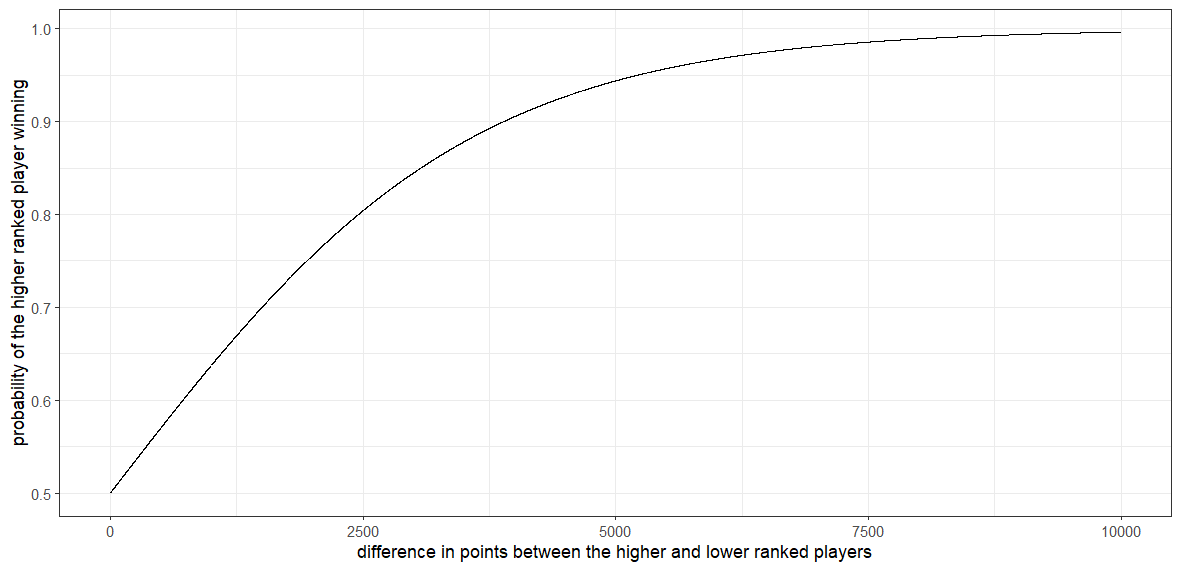
\includegraphics[scale=0.6]{images/logistic_curve.png}
  \caption{Point Difference v Probability}
  \label{fig:logisticcurve}
\end{figure}
This parameter was found to be $\theta = 0.000565$. As a
result of this the Logistic Model can be defined as follows.
\begin{gather}
  \pi_i = -\dfrac{1}{1+e^{-0.000565D_i}}
\end{gather}
Applying this model
to each match where both players have rank points will generate the results
required to calculate both accuracy and log loss. As well as this,
altering the threshold to only provide a prediction if the calculated probability
is over a certain threshold will be implemented. Testing a range of threshold
values will inform what value provides the best balance of providing predictions
to as many matches as possible whilst maintaining a high level of confidence in the
predictions. This work will be expanded in the future work section of this report.

\subsection{K Factor Model}
Adjusting the value of the K value in the K Factor model will involve iterating
over various values of K to identify any differences in accuracy and log loss
that come with shifting these K values. Initially the value was set to 5,
however once a broad grid search was completed as outlined in the results section
selected value for K was set to 30.

\subsection{Five Thirty Eight Model}
Similar to the K Factor model various values for $\delta$, $\nu$ and $\sigma$
were iterated over. Since there are three parameters that can be tuned
the search space will need to be reduced when compared to the K Factor model.
Like the K Factor model, a brute force approach was completed to find near optimal
hyperparameters as outlined in the results section. The found near optimal parameters
were very close to known optimal values \cite{kovalchik_searching_2016}
The values were set to $(\delta,\nu,\sigma) = (240,5,0.4)$.

\subsection{Surface Augmented Five Thirty Eight Model}
An extension to the Five Thirty Eight model was implemented which calculates a set of
Elo scores for each player on each surface. These scores are calculated using the
Five Thirty Eight model by calculating a probability that each player would win on the
given surface. This probability is then used to update the Elo rating fore each player
on the given surface. As a standalone model, these surface Elo ratings capture such a
small amount of information that prediction ability is minimal. These surface Elo's were
combined with the base Five Thirty Eight model as an augmentation.
The optimal method of combining these surface models was investigated. A defined weighting
value $\gamma$ was used to influence what proportion of the final model output was
the Five Thirty Eight model and what was the Surface model. The first approach of
combining these models was taking the calculated probability of player 1 winning, $p_1$,
from each models and combining them to generate a new probability $p_{1,c}$ based
on the weighting factor
\begin{gather}
  \pi_{1,c} = \gamma*\pi_{1,f} + (1-\gamma)*\pi_{1,s}
\end{gather}
where $\pi_{1,f}$ is the Five Thirty Eight Elo probability of player 1 winning and
$\pi_{1,s}$ is the Surface Elo probability of player 1 winning.
The other approach was to combine the Elo scores produced by each model for each match
using the $\gamma$ weighting factor with the Five Thirty Eight Elo rating at match $T$
defined as $E_{f}(T)$ and the surface Elo at match $T$, $E_{s}(T)$,
the combined Elo rating, $E_{c}(T)$, can be calculated using the $\gamma$ value As
\begin{gather}
  E_{c}(T) = \gamma*E_{f}(T) + (1-\gamma)*E_{s}(T)
\end{gather}
Then using the same formula from (3) to calculate $\pi_{ij}$ the probability of player
1 beating player 2 can be found
\clearpage
\section{Results}
After building and testing the different models, the metrics for each have been displayed
in Table 1. In the following section the methods for optimising the resulting metrics
will be explored. From Table 1 it can be observed that the best performing model was the
Bookmakers Consensus model with the highest accuracy and lowest log loss. Although it did
have a marginally worse calibration. Out of the models appropriate for predicting match
outcomes, the Surface Combined Elo models performed the best with the different methods for
including the surface information resulting in a negligible difference in calculated metrics.
\begin{table}[h]
  \begin{tabular}{||c c c c||}
    \hline
    Model                                     & Accuracy & Log Loss & Calibration \\
    \hline\hline
    Higher Rank                               & 0.660    & NA       & NA          \\
    Logistic Regression                       & 0.639    & 0.634    & 0.867       \\
    K Factor                                  & 0.658    & 0.613    & 0.889       \\
    Five Thirty Eight                         & 0.662    & 0.614    & 0.897       \\
    Surface Elo                               & 0.598    & 0.722    & 0.944       \\
    Five Thirty Eight - Surface Combined Elo  & 0.663    & 0.614    & 0.893       \\
    Five Thirty Eight - Surface Combined Prob & 0.663    & 0.612    & 0.892       \\
    Bookmakers Consensus                      & 0.695    & 0.575    & 0.863       \\
    \hline
  \end{tabular}
  \caption{Metrics for all investigated models showing that the best performing model was
    the Bookmakers Consensus and the best overall predictive model being either of the
    Surface Combined Elo models}
\end{table}
\subsection{Logistic Model}
Running the logistic model provides the bElow output
\begin{table}[h]
  \centering
  \begin{tabular}{||c c c c c||}
    \hline
    Accuracy & Log Loss & Calibration & Correct & Incorrect \\
    \hline\hline
    0.639    & 0.634    & 0.867       & 68084   & 38486     \\
    \hline
  \end{tabular}
  \caption{Generated metrics for the Logistic Regression Model}
\end{table}

For an overall accuracy value of 0.639. The corresponding log loss for this model is 0.634.
With an accuracy lower than simply using the player ATP rank to predict the outcome of a
match the model in this form has definite room for improvement. Since the predictions of
this model in its current form is based solely on the difference between the players rank
points it can be observed that the accuracy of its predictions are similar to using the ATP
rank. In the future work section, capturing more features of the dataset to include in the
logistic model will be done which is an extension not possible with simply using the players
ATP rank.
\subsection{K Factor}
The K Factor model provides one parameter that can be adjusted to alter the models' performance.
This K value impacts both the accuracy and the log loss produced from the model. The table
bElow shows the accuracy and log loss for each value of K.

\begin{table}[h]
  \centering
  \begin{tabular}{||c c c||}
    \hline
    K Value & Accuracy & Log Loss \\
    \hline\hline
    5       & 0.639    & 0.631    \\
    10      & 0.648    & 0.619    \\
    15      & 0.653    & 0.614    \\
    20      & 0.655    & 0.613    \\
    25      & 0.657    & 0.612    \\
    30      & 0.658    & 0.613    \\
    35      & 0.657    & 0.615    \\
    40      & 0.658    & 0.620    \\
    45      & 0.659    & 0.623    \\
    50      & 0.659    & 0.627    \\
    \hline
  \end{tabular}
  \caption{K value tuning to find the optimal value based on Accuracy and Log Loss, It
    can be observed that the optimal value is K=30}
\end{table}
From the results above it can be observed that as the K value increases, the log loss decreases.
This, however, corresponds with a decline in the models overall accuracy. As this model
does not consider the past performance of the players when updating their corresponding
ranks potential improvements to this model are minimal. The following plot tracks the performance
of Roger Federer across his long career.

\begin{figure}[H]
  \centering
  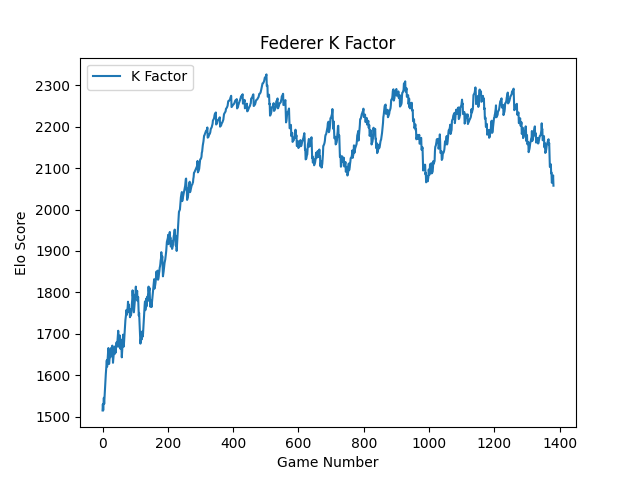
\includegraphics[scale=0.8]{images/federer_k_factor.png}
  \caption{K Factor Federer Rank Over Time}
  \label{fig:federer-kfactor}
\end{figure}

It can be observed the model captures the trajectory of his career quite well with a rapid increase
in his rank early in his career, an extended peak
during the middle of his career coinciding with his "prime" and then as his score approaches the lowest
value of his prime his retirement.

\subsection{Five Thirty Eight Model}
As mentioned in the Method section of this report the Five Thirty Eight model relies on
three hyperparameters to define the model. The values $(\delta,\nu,\sigma) = (240,5,0.4)$
were determined after completing a broad grid search across all permutations for $\delta$
between the values of 100 and 300 with a step increment of 20, $\nu$ between the values of
1 and 10 with a step increment of 1 and $\sigma$ between the values of 0.1 and 1 with a
step increment of 0.1. This involved building and testing a thousand different models
and generating summary statistics for all of them. Although more advanced methods of
hyperparameter tuning could have been implemented the results of this broad grid search
showed that the optimal values for accuracy and log loss were maximised at the given values
and align closely with values published in existing literature \cite{kovalchik_searching_2016}

Running the Five Thirty Eight model with these parameters provides an accuracy value of
0.662 and an overall log loss of 0.614. This shows higher accuracy when compared
to the K Factor model
with a lower corresponding log loss value implying a higher confidence in the models predictions.
Similar to the K Factor result, the career ranking of Roger Federer has been plotted bElow.

\begin{figure}[H]
  \centering
  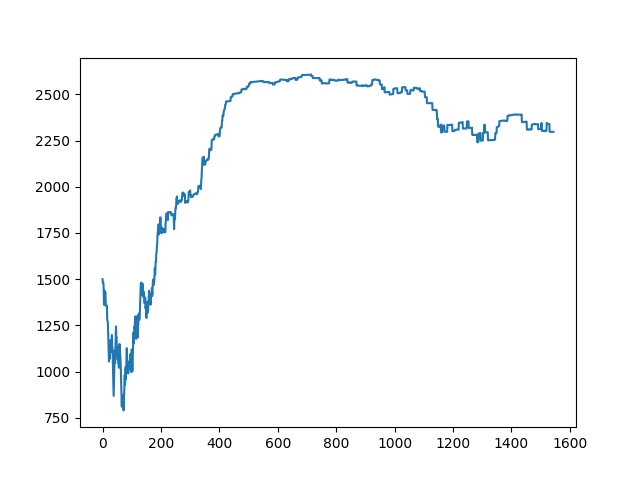
\includegraphics[scale=0.8]{images/federer_538.png}
  \caption{Five Thirty Eight Federer Rank Over Time}
  \label{fig:federer-538}
\end{figure}

This plot looks almost identical to the K Factor ranking for Federer which explains why
accuracy of the models is quite similar. The Five Thirty Eight model has Federer having a
higher peak rating with a marginally higher rate of change when outlier performances occur.

\subsection{Surface Combined Five Thirty Eight Model}
As discussed in the method section, the existing Five Thirty Eight model was augmented
with a separate Elo rating generated for each player on each surface type. From Table 1
it can be observed that the Accuracy was identical for both methods of combining the models
sitting at $0.663$ with Log Loss and calibration both having a negligible difference
$\approx 0.002$. When looking at the Surface Elo model that hasnt been combined with an
optimised Five Thirty Eight model, it can be observed that its performance is significantly
worse than any of the other models in all metrics excluding calibration. Discussion into why
this is the case will be done later in this report.

\subsection{Bookmakers Consensus Model}
The Bookmakers Consensus model outperformed all the other models significantly in accuracy
and log loss with values of 0.695 and 0.575 respectively. The natural question that follows
from the results of this model is why is this not the model selected as the best for
predicting tennis match outcomes? For reasons that will be explored on in the discussion
section of this report, due to how the information for each match played is reported, this
model cant be used until after a match is played making it unsuitable as a solution for
the prediction problem.

\subsection{Match Subset Investigation}
To dive deeper into the behaviour of the individual Elo models, a random subset of a single players
matches were selected from the data and the Elo scores for each of those matches were
plotted. Roger Federer was the player selected and his 300th to 330th games were used.
The bElow plot was generated.

\begin{figure}[H]
  \centering
  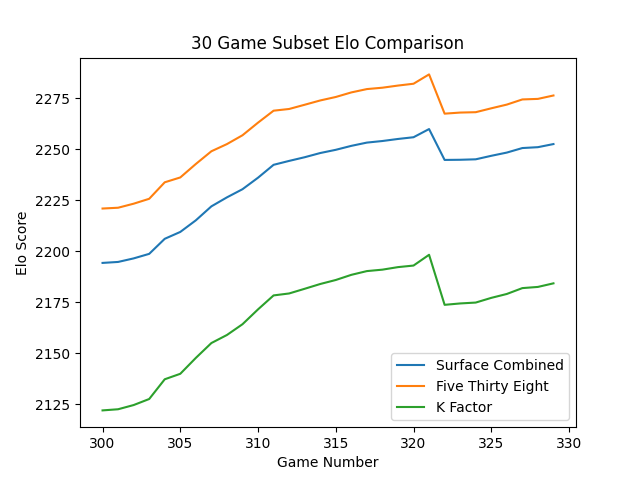
\includegraphics[scale=0.8]{images/30_game_subset.png}
  \caption{Federer 30 game subset}
  \label{fig:federer-30}
\end{figure}

From Figure 4 it can be observed that the models have the same trajectories across the
various Elo models which is to be expected. If a player wins a game the score should go
up and if a player loses the game the score should go down. Where the models differ is
in the magnitude of change.
\\
\begin{table}[H]
  \begin{tabular}{||c c c c c c c c||}
    \hline
    Winner    & Loser      & Surface W & Surface L & 538 W & 538 L & K W  & K L  \\
    \hline\hline
    Federer R & Agassi A   & 2259      & 2021      & 2286  & 2028  & 2198 & 1919 \\
    Safin M   & Federer R  & 1982      & 2244      & 2030  & 2267  & 1937 & 2173 \\
    Federer R & Ulihrach B & 2244      & 1583      & 2267  & 1611  & 2174 & 1519 \\

    \hline
  \end{tabular}
  \caption{Elo model scores for match between Federer and Safin where Federer lost.
    Including Federers games immediately before and after.
    This figure highlights the impact the differences between the models when calculating
    Elo score changes}
\end{table}
Table 4 shows the differences in both the starting Elos of each player in the game of
interest and the change of Elo caused by the loss.
It can be observed that the models are in lockstep whilst
Federer is winning, however when Federer loses game 321 the K model heavily punishes
his score as it does not take into account his history of winning and solely focuses on
the difference in player scores and K value to determine the amount to reduce the score.
The Five Thirty Eight based models still punishes his score due to the loss, however at a
lower rate. The Surface Combined Elo has the smallest drop of all the models which is most
likely due to Federer having a lower Surface Elo for that match resulting in a reduction
of his combined Elo score. This would correlate to a smaller drop as the difference in
rating is smaller.

\subsection{Federer Career Investigation}

The current implementations of the various Elo models captures a similar trajectory in a
players career. This can be observed by overlaying the three Elo models which are updated
on a game by game basis, K Factor and Five Thirty Eight.
\begin{figure}[H]
  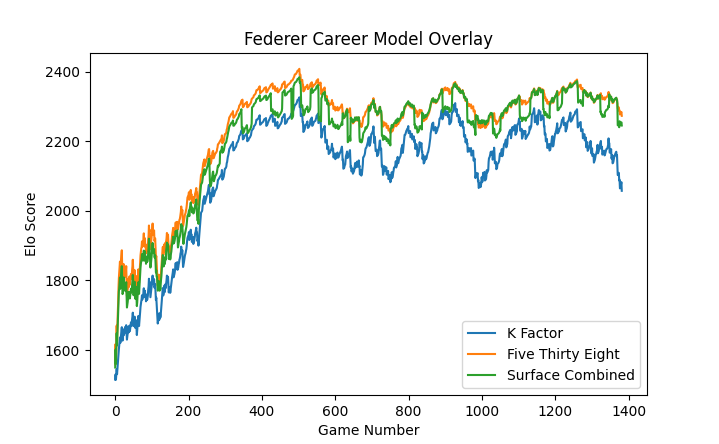
\includegraphics[scale=0.8]{images/federer_career.png}
  \caption{K Factor, Five Thirty Eight and Surface Combined Elos}
  \label{fig:federer-k-538}
\end{figure}

From Figure 5 it can be observed that the Five Thirty Eight Model varies more than the
K Factor model as a result of individual matches. This is because it considers the players
history when determining a K value for the rank update. Outlier performances have a greater
impact on an individual update which results in a lower rating being assigned early in the
career with poorer performances occurring. Conversely, as Federers performance increases,
the improvement is picked up earlier in the Five Thirty Eight model when compared to the
K Factor model. This results in the model reaching a steady state that accurately reflects
Federers skill earlier than the K Factor model which when optimal parameters are identified
should result in a higher overall accuracy. The Surface Combined model sits between the
K Factor and the Five Thirty Eight models with the variance in rankings increased when compared
to the base Five Thirty Eight model. This is caused by the influence of the highly volatile
surface Elo of the player. Since the two ratings are combined using the weighting factor there
are two points in which an upset could occur resulting in the potential for more volatile
rating changes.

\vspace{10mm}
\noindent \hrulefill

\clearpage
\section{Discussion}
From the results of the initial implementations of these models there is some key
takeaways. The basic logistic model has the lowest accuracy meaning that it
makes the least correct predictions. Interestingly the accuracy of the logistic model is
worse than simply predicting the higher ranked player to win any given game. This could be
caused by games dropped from the dataset as a result of the merging process.
In its current state this logistic model currently only
considers a single parameter, the players rank points, however there is opportunity to
extend this model to include other parameters present in the dataset. This work will be expanded
on in the future work section of this report.

The naive option of picking the higher ranked player to win any given game turns out to have
a reasonably high accuracy with 0.660. The only predictive models that outperform it are the base
Five Thirty Eight model and the Surface Combined model. The K Factor and Logistic Regression models
perform worse, however due to the probabilistic functionality of these models log loss and calibration
metrics can be obtained to more accurately measure their performance. The basic K Factor model
is as optimised as it can be after the investigation to find the optimal K value was completed.
There is still opportunity to optimise the Logistic Regression model through incorporation of
other parameters in the model. Due to the current poor performance of the model when using
the difference in rank points, an important statistical feature of the dataset, it is highly ulikely
that this work would result in a model that performs as well as the other Elo models.

The Five Thirty Eight model performs quite well with a better accuracy than the naive approach and
comparable log loss and accuracy to the best performing predictive models. The Five Thirty Eight
was the most influential model that was built and trained as it was used individually and as a
part of the Surface Combined Elo models. The broad grid search to find the optimal hyperparameters
was chosen over the more complex options such as gradient descent as it was observed that the
performance metrics of the various values did not change by much when they were close to the found
near optimal values. Due to the complexity of implementation on minimal potential for metric
improvement the simpler grid search was determined to be sufficient for this report. The optimal
values for the Five Thirty Eight model were used to build the standalone surface Elos for each
player and there is the potential that these values were not the most optimal. The impact of this
is negligible since the weighting factor used when combining the two models heavily reduced the impact
of the individual surface Elo on the final rating. The optimal weighting factor was found to be 0.85
therefore the impact of any sub optimal hyperparameters would be reduced. In the future work
section the hyperparameter tuning for the surface Elo will be conducted to investigate if there is
some unexpected performance gains that can be achieved.

Combining the surface model with the Five Thirty Eight model resulted in an overall better performing
model with accuracy and log loss being improved however a slightly lower calibration value.
The differences in the metrics were minor implying that overall the combination of these two models
did not demonstrate significantly different behaviors and only had an impact on prediction when the
base Five Thirty Eight ratings for each player were extremely close. Since the majority of games
are played on a hard surface, the surface Elo may not be adding much value to predictions made on
this surface. Performance on the most common surface type should not vary as much between players
resulting in a rich get richer scenario where the top performing players have a high surface Elo
on the hard surface since they win many games on that surface. Figure 5 highlighted this issue with
the surface Elo impacting the overall rating for Federer greatly when he loses to newer players.
Since the underlying Five Thirty Eight model is unbounded and Federers surface Elo rating is
extremely high, the Elo drop that results from losing the match is enormous, even with the weighting
factor. Mitigations for this will be explored in the future work section. The
potential of only incorporating the surface Elo when played on the more volatile surfaces, grass
and clay, will also be investigated.

When comparing the predictive model results to the BCM as a benchmark model
it can be observed that there is room for improvement. The BCM vastly
outperforms the all the models in both accuracy and log loss. It does have a worse calibration
value which is to be expected due to the incentives present inherent in the BCM. It can be assumed
that betting companies value the log loss metric higher than all other metrics as it implies a level
of confidence in predictions and there is a strong profit incentive in not being wildly wrong
in any given prediction. Since bookmakers odds for given matches aren't collated prior to a match
being played, this model is inappropriate for predicting future matches. There is potential for
writing a system that scrapes and collates these odds from either the bookmakers websites or
certain odd aggregation websites. There are potential issues with building and using a system like
this without permission as there is potential that they go against the terms of service of the
various sites and can have ramifications around copyright resulting potentially resulting in
sanctions being placed on the user \cite{out-lawcom_ryanair_nodate}

\subsection{Future Work}
Extending the investigated models will be the focus for the next part of this research
project. Starting with the logistics model the natural extension of the current model
is to investigate additional parameters to include. Utilising the R logistics model
package, both additional parameters and interaction terms will be tested for statistical
significance to the match outcomes. Incorporating playing surface and playing hand will
be investigated first as there is some evidence that it can have an impact on match
outcome \cite{loffing_left-handedness_2012}.

The basic K Factor Elo model will not be investigated any further as the various values
of K and its impact on model performance have already been investigated above. The Five
Thirty Eight model leverages three independent hyperparameters to calculate the change
in ranking after each contest. Although using a brute force solution for determining near
optimal hyperparameters was conducted a more sophisticated solution will be investigated to
see if better values can be found. There are many methods of optimisation for
hyperparameter search \cite{claesen_hyperparameter_2015} and investigating the
most appropriate one for optimising the Elo model parameters will form the basis of
future work for improving the Five Thirty Eight model. This process will also be completed
for the standalone surface Elo's since no investigation has been completed on the impact of
using the current Five Thirty Eight parameters for this model.
Due to the volatility in the Surface Rating Elo an investigation will be done to determine
whether bounding the maximum rating change will increase model performance. This will either
be achieved by setting a maximum rating change for the Surface Combined Elo or by modifying
the hyperparameters of the underlying Five Thirty Eight model. Finding the optimal hyperparameters
for the Surface Combined Elo will need to utilise more robust tuning methods than a broad search
since the interaction between the Surface and the Five Thirty Eight Elo can have an impact of the
optimal parameters.

The current method of determining whether any of these Elo models have produced a correct
prediction is by determining if the probability of player i beating player j is greater
than 0.5. Logically this is a good starting point as it implies that theres is a greater
than 50\% chance of a player winning. Setting this probability threshold to different values
will be investigated further to identify any improvements in the models prediction accuracy.
With a higher threshold, it is expected that the model will make predictions on less
matches as when players have similar Elo scores the model will not make a prediction.
Balancing the improvement to model accuracy versus the reduced number of matches in which
a prediction is made will be completed and discussed.

Weighting the Elo rating changes based on the level of match played will be another area of
investigation. Currently all matches are treated equally however it may be beneficial to weight
matches played in grand slams higher than matches played in lower level tournaments. The WTA ranks
do something similar with the maximum points varying based on the level of the given tournament.
This idea can be extended with extra weighting being given for higher rounds. Ie the Elo rating
change should be higher if a player wins the final match in a grand slam.
\clearpage

\section{Conclusion}
Performance of these models have been quantified by measuring both
model accuracy and the log loss of the models predictions. There are many mathematical models that can be applied to the tennis prediction problem.
These models range in both complexity and performance as such robust performance testing
has been conducted to identify which models perform the best. Performance of these models
have been quantified by measuring model accuracy, log loss and calibration of the models
predictions. Extensive open-source datasets of historical tennis data was leveraged to
both build and test these models. Currently a small subset of the available data is being
used to build these models. Future work will include incorporating a greater number of
features within the dataset. Capturing more features of the available data and conducting
statistical analysis on its impact on match outcome will result in more accurate predictions
with a higher confidence as measured by its corresponding log loss value.

The logistic model performs well with just a basic classifier based on a
players ATP rank. The log loss of the logistic model, is higher than other models
investigated in this report. This implies that the model,
confidence in its predictions is lower than alternatives such as the Elo models.
Attempting to address this issue will be conducted as a part of future work by
extending the parameters used to build the logistic model to increase the models
confidence in its predictions.

Various Elo models were implemented and their respective performances compared. These Elo
models have better performance than the basic logistics model with a
lower log loss value. Differences in the ratings' of an individual player
generated by the individual models shows that they all succeed in capturing the overall
trajectory of a players career. The different Elo models update the player ratings at
different rates based on performance. Having the model accurately update these ratings
is the key to maximising accuracy whilst minimising log loss.

\clearpage

\bibliographystyle{plain}
\bibliography{bib_file}

\vspace{10mm}
\noindent \hrulefill

\end{document}


